\chapter{Introduction}
\label{intro}

\section{Cryptography} % around 3/4 pages
Cryptography is a mathematical science for encryption and decryption of
data. The meaning of the data should therefore be hidden to anyone who must
not understand it, but should become understandable to whom the data is
sent to.\newline
Cryptanalysis is the complementary of the cryptography
with the focus on the defeat of the cryptographic mathematical
techniques.\newline
Both terminology is named cryptology.

The most important security of the information is defined into:
\begin{itemize}
  \item Confidentiality or privacy\newline
  No one, except whom is intended, can understand the transmitted data
  \item Integrity\newline
  No one can alter the transmitted message without the alteration is being
  detected
  \item Authentication \newline
  The sender and the receiver can identify the destination of the data and
  identify themselves
  \item Non-repudiation\newline
  The sender cannot deny at a later stage the transmission of the datas\newline
\end{itemize}
The cryptographic mathematical techniques are grouped into several algorithms:
\begin{itemize}[noitemsep]
  \item Hash algorithm
  \item Signature algorithm
  \item Symmetric cipher algorithm
  \item Asymmetric cipher algorithm
\end{itemize}

\subsection{Hash algorithm}
\label{intro_hash}

Hash functions are widely used in several other cryptographic
algorithms, as signature or cipher.
A digest, which is a short, fixed-length bit-string, is the result of a computed
message over a hash function.
This digest is considered practically impossible to invert, meaning
that impossible to recreate the input data with it.
The main properties of a hash function are:
\begin{itemize}[noitemsep]
  \item it's quick to compute the digest for any message
  \item it's infeasible to generate a message from its digest
  \item it is infeasible to modify a message without changing the digest
  \item it is infeasible to find two different messages with the same
  digest.\newline
\end{itemize}

Several hash algorithms are used today, with different properties shown on table
\ref{tab:intro_hash}. 

\begin{center}

\begin{tabular}{| c | *{4}{c|}}
 \hline
 Algorithm 	& Output & Input & Collisions \\
           	& (bit)  & (bit) & found		 \\
 \hline
 MD5 	   	& 128	& 512	& yes \cite{RFC7465} \\
 SHA1	   	& 160	& 512	& not yet \\
 \hline
SHA-224		& 224	& 512	& no \\
SHA-256		& 256	& 512	& no \\
SHA-384		& 384	& 1024	& no \\
SHA-512		& 512	& 1024	& no \\
\hline
 
\end{tabular}
\captionof{table}{Properties of hash algorithms}
\label{tab:intro_hash}

\end{center}

\subsection{Digital signature algorithm}
\label{intro_sign}

Digital signatures are one of the most important cryptographic algorithms that
are widely used today. Digital signatures can be used with public key
cryptography (asymmetric key, see section \ref{intro_asym_cipher}), which
provides authentication, the receiver can verify the authenticity of the
incoming information, and data integrity, the receiver can verify that the
informations are intact.
One of the most important properties of digital signature is that it provides
non-repudiation, meaning that the sender cannot claim he has not sent the
data.

\begin{figure}[!ht]
\centering
%\frame{
% trim: left, bottom, right, up
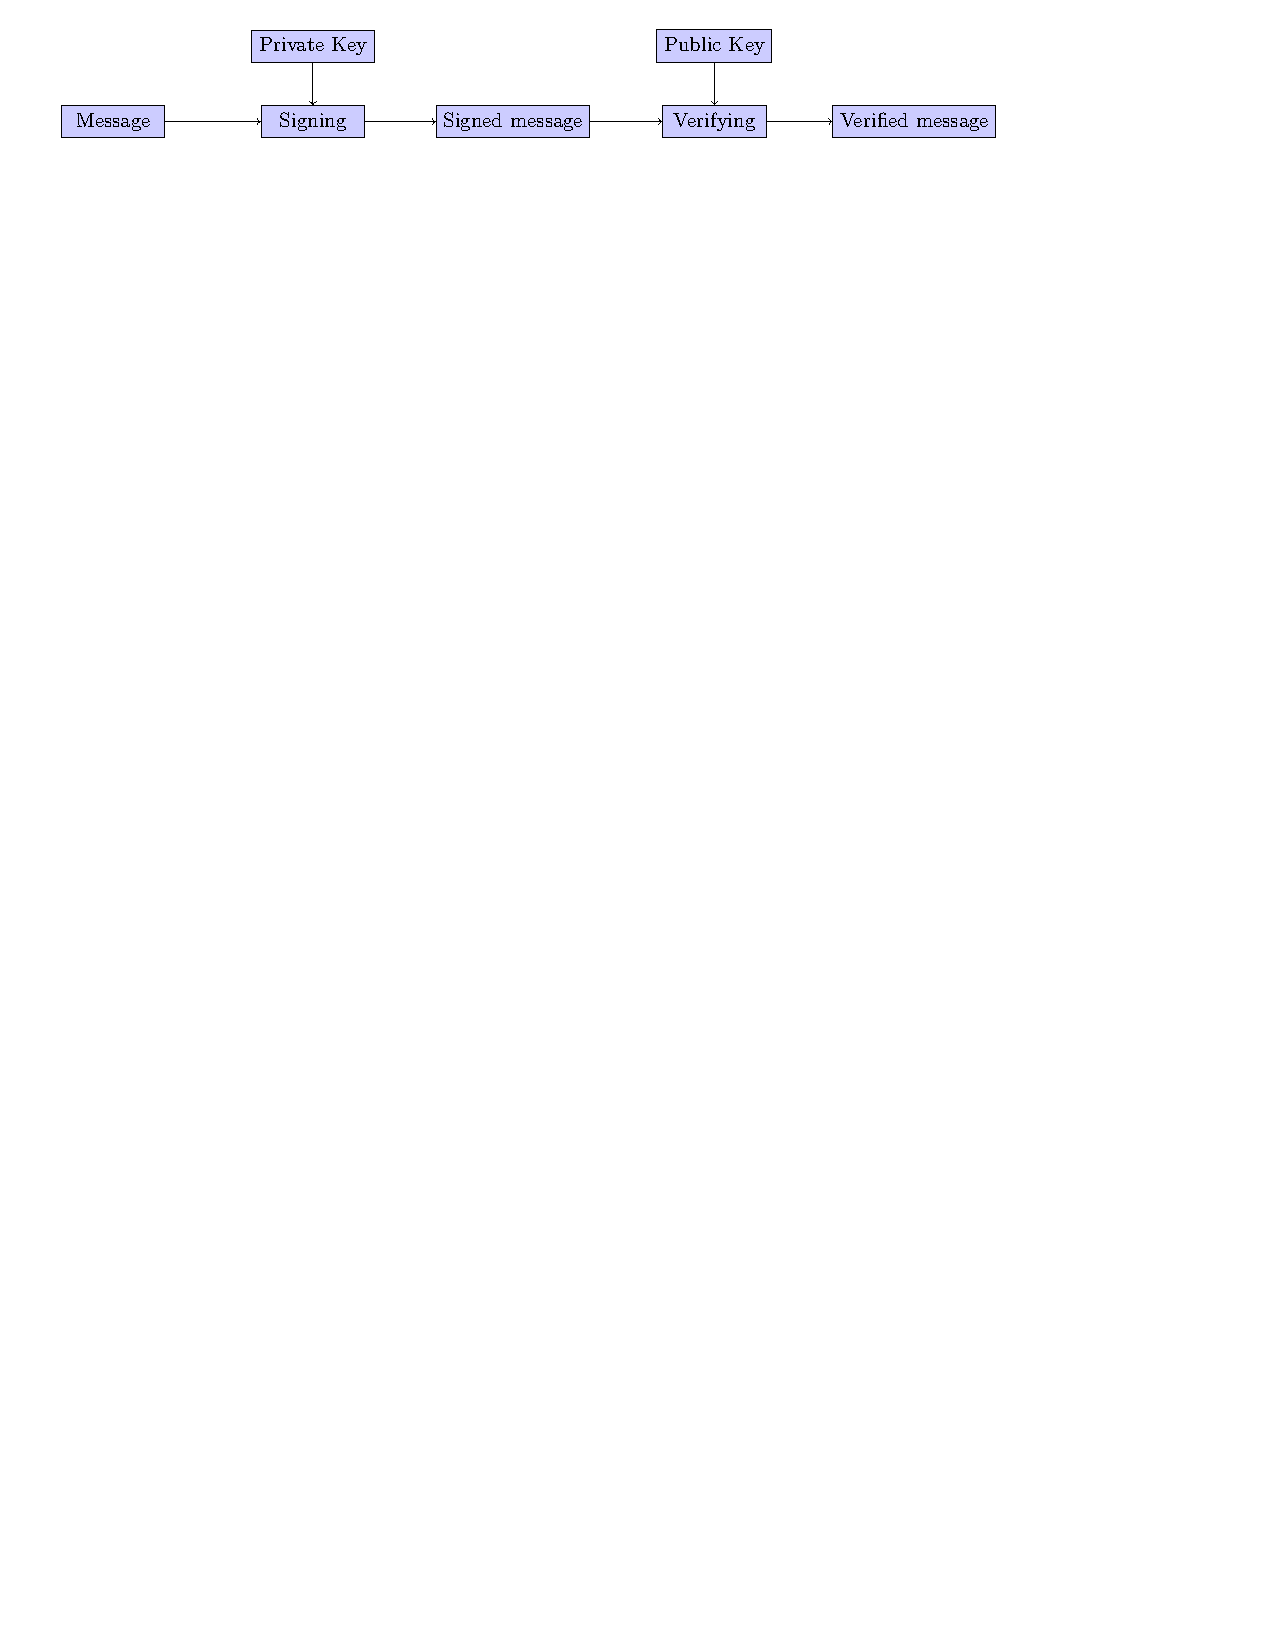
\includegraphics[trim=2cm 25.5cm 5cm 0cm,
height=2.5cm]{figures/intro_signature.pdf}
\caption{Introduction of a signature operation}
\label{fig:sign}
%}
\end{figure}

As shown on the figure \ref{fig:sign} a message, which could previously be
hashed, is signed with the private key, which only one person has it.
The signature can then be verified with the public key, which should be
generated with the private key used to sign the message.

Three types of digital signature are available:
\begin{itemize}
  \item RSA signature scheme, which is the most widely used digital signatures
  scheme in practice.\newline
  The Probalistic Signature Standard (PSS) RSA Padding \cite{RFC3447} should be
  used to increase the security of the signature. This padding is a signature
  scheme based on the RSA cryptosystem (see section \ref{intro_secu}) and
  combines signatures and verifications with an encoding of the message (see
  section \ref{intro_asym_cipher}). It allows to the receiver to distinguish
  between valid and invalid messages.
  \item DSA signature scheme \cite{RFC6979}, which is a variant of the Elgamal
  signature \cite{wiki:elgamal}
  \item ECDSA signature scheme \cite{RFC6979}, which is closely related to the
  DSA scheme, but constructed in the group of an elliptic curve
  (see section \ref{intro_secu}).
\end{itemize}

The security provides by each signature scheme is explained in section
\ref{intro_secu}.

\subsection{Message Authentication Code (MAC)}
\label{intro_mac}

The Message Authentication Code (MAC) is widely used in practice. It has some
properties with digital signatures (see \ref{intro_sign}), since it provides
message integrity and message authentication, but do not provide
non-repudiation, because of the use of symmetric keys.
MAC is much faster than digital signatures since it's based on block ciphers or
hash functions.

\begin{figure}[!ht]
\centering
%\frame{
% trim: left, bottom, right, up
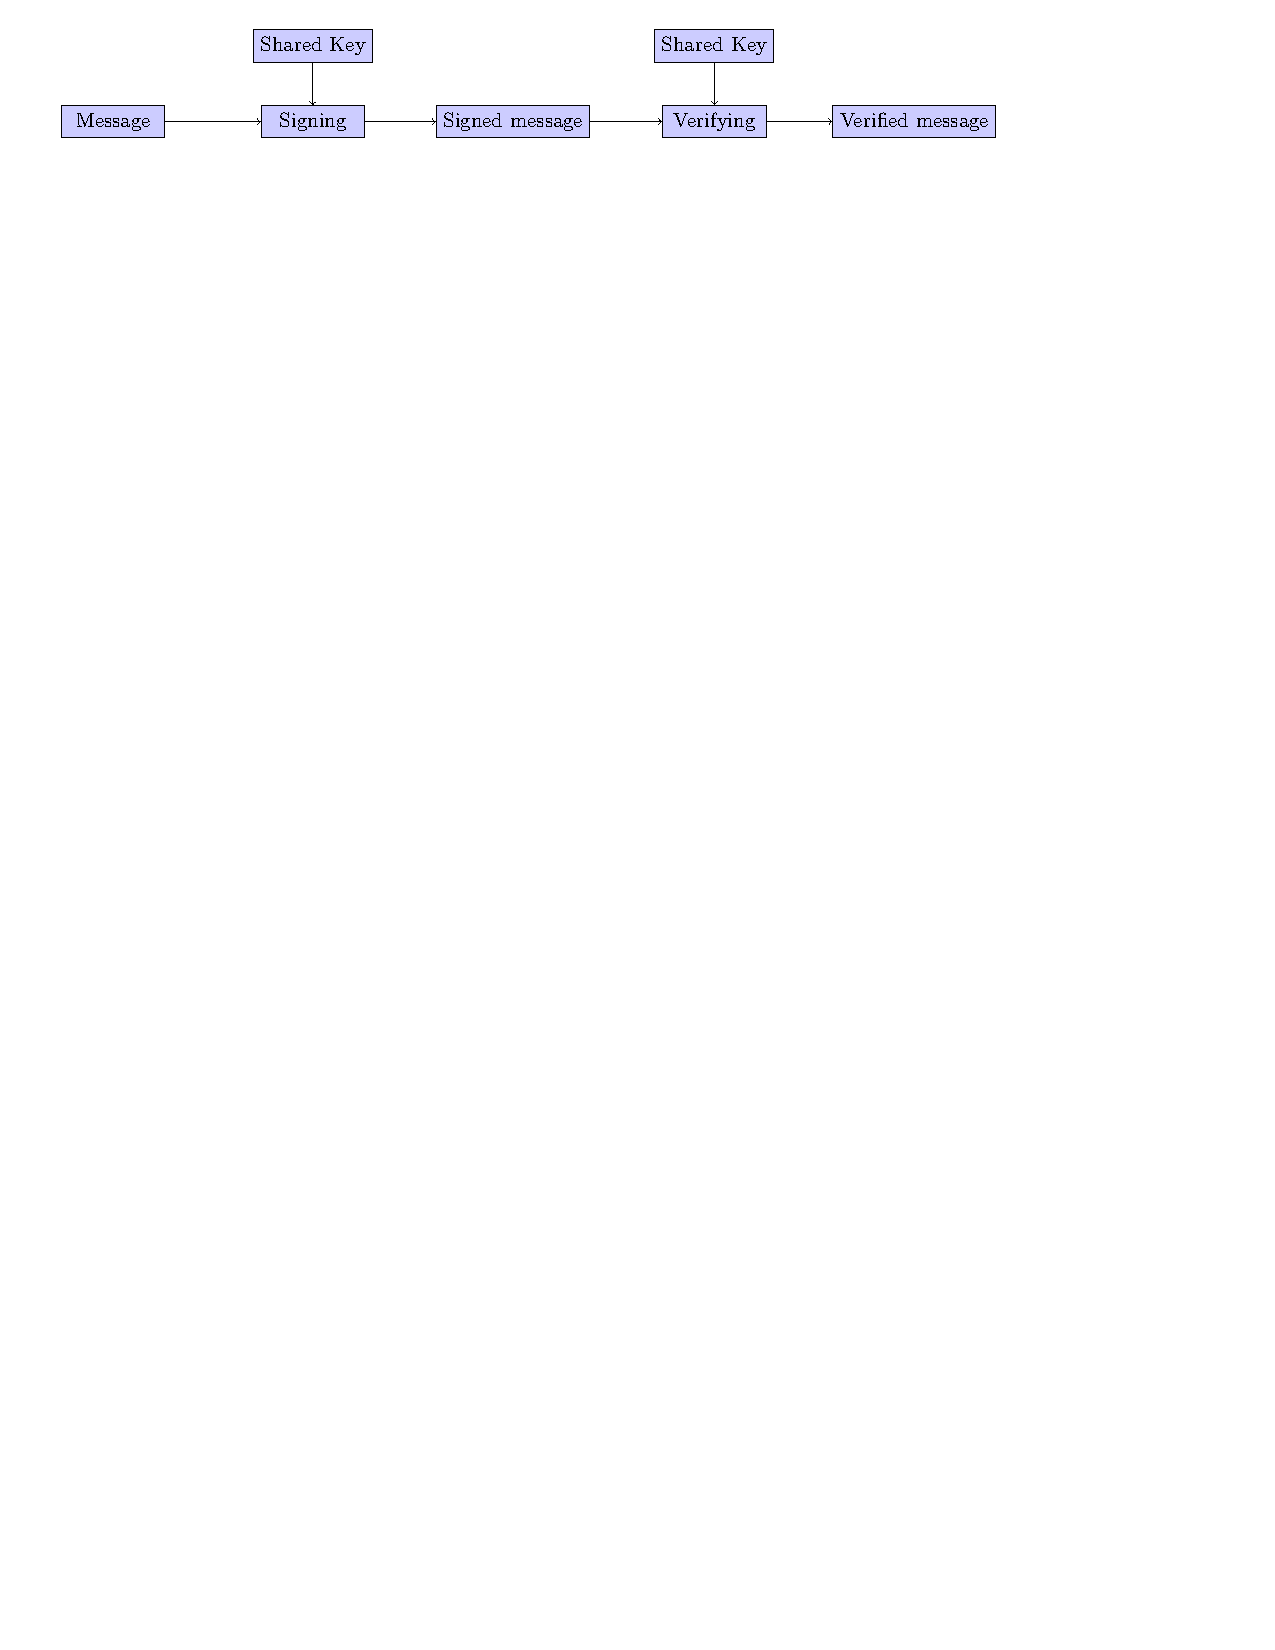
\includegraphics[trim=2cm 25.5cm 5cm 0cm,
height=2.25cm]{figures/intro_mac.pdf}
\caption{Introduction of a MAC operation}
\label{fig:mac}
%}
\end{figure}

As shown on figure \ref{fig:mac} MAC uses symmetric keys for both generating and
verifying a message.

The properties of a MAC are:
\begin{itemize}
  \item Cryptographic checksum\newline
  Secure authentication tag for a given message (when use with hash functions)
  \item Symmetric\newline
  Signing and verifying are done with symmetric keys
  \item Arbitrary message size\newline
  The input can be of different sizes
  \item Fixed output length\newline
  The signature generated by the MAC has a fixed output length
  \item Message integrity\newline
  Any modification of the message during the transit will be detected by the
  receiver
  \item Message authentication\newline
  The receiver is ensured of the origin of the message
\end{itemize}

The two mains MAC are:
\begin{enumerate}[noitemsep]
  \item MAC from Hash functions (HMAC) \cite{wiki:hmac}, which is a hash-based
  message authentication code 
  \item MAC from Block Ciphers (CBC-MAC) \cite{wiki:cbcmac}, which is a block
  cipher-based message authentication code
\end{enumerate}

\subsection{Cipher}
\label{intro_cipher}

 The cipher is an algorithm uses for encryption of data (plaintext) and
 decryption of data (ciphertext).
 It's used on the internet, for the e-mail, on cellphones when calling, etc.
 Two main cipher algorithms exist, which are:
 \begin{itemize}[noitemsep]
   \item Symmetric cipher algorithm
   \item Asymmetric cipher algorithm
 \end{itemize}


\subsubsection{Symmetric cipher algorithm}
\label{intro_sym_cipher}

\begin{figure}[!ht]
\centering
%\frame{
% trim: left, bottom, right, up
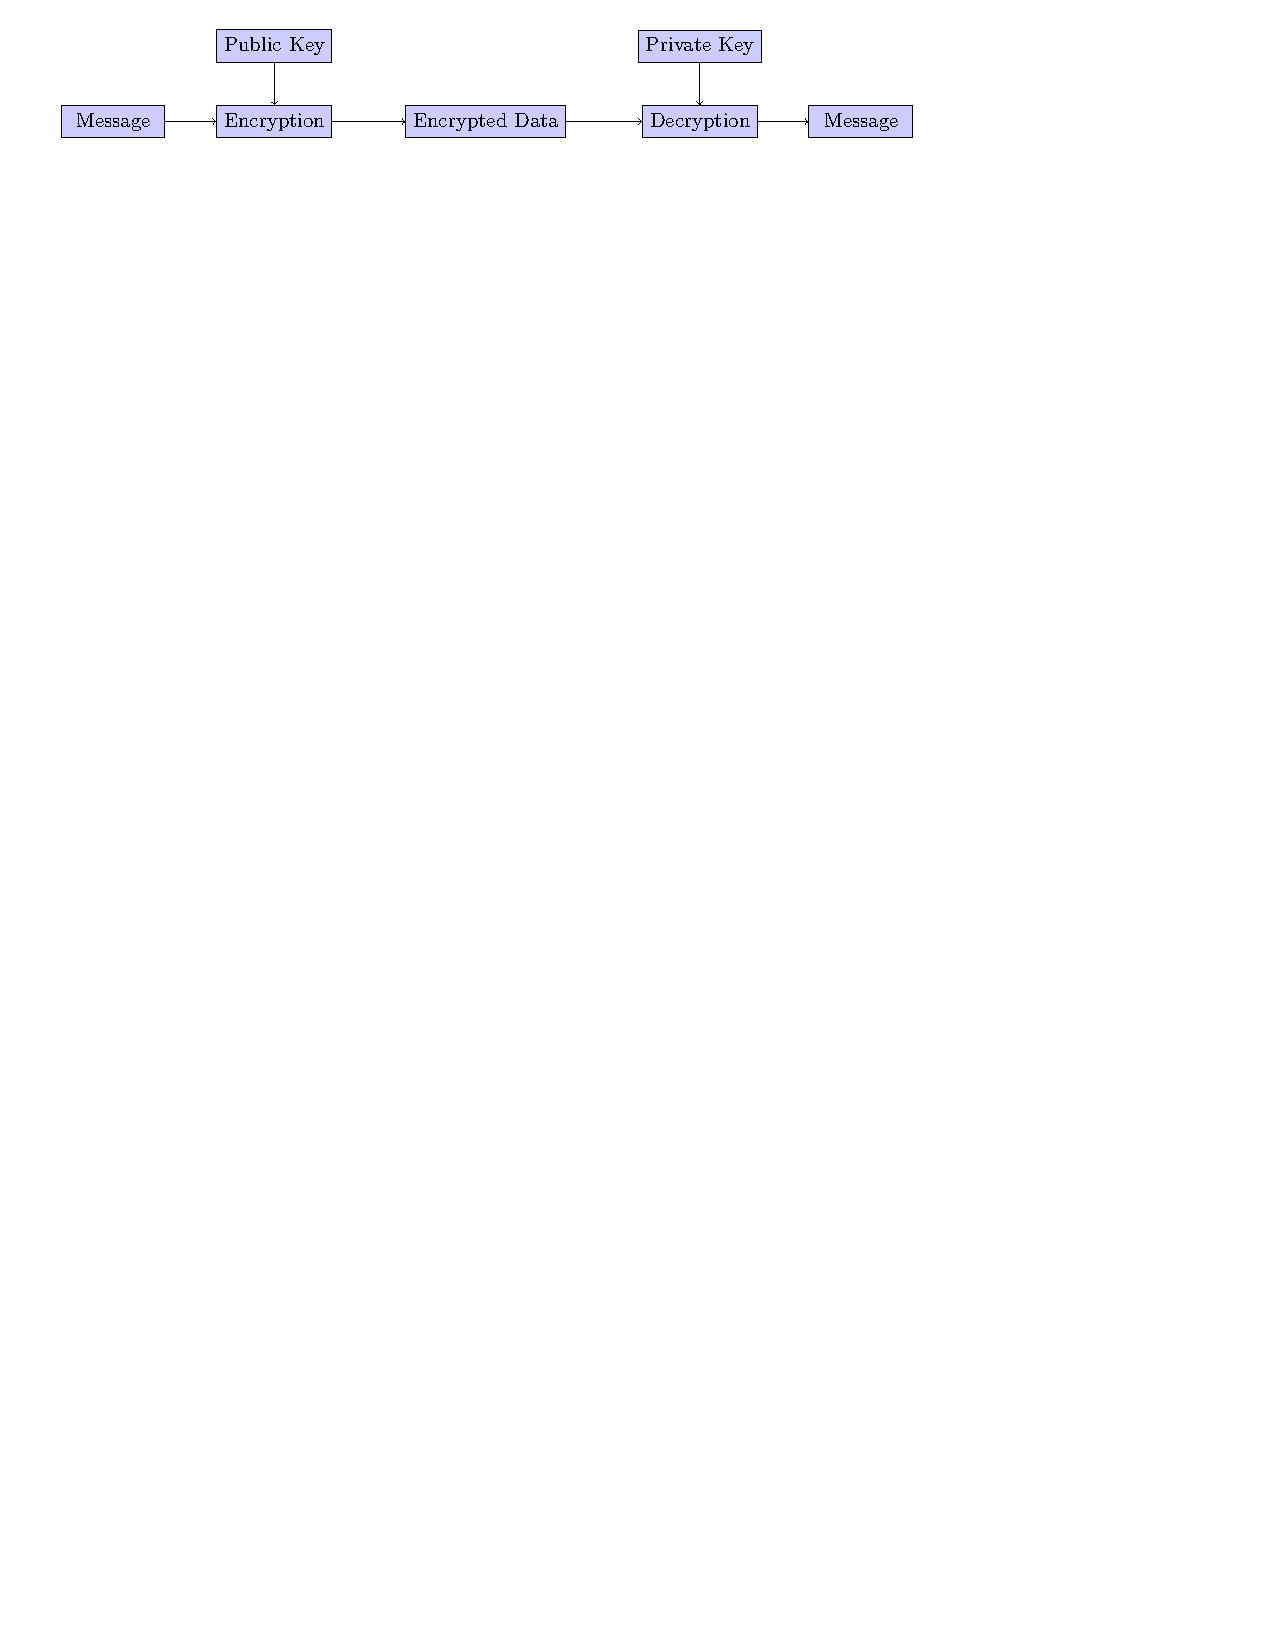
\includegraphics[trim=0cm 25.25cm 5cm 0cm]{figures/intro_sym_cipher.pdf}
\caption{Introduction of a symmetric cipher operation}
\label{fig:sym}

%}
\end{figure}

Symmetric-key algorithms are algorithms for cryptography that use the same
cryptographic keys for both encryption of plaintext and decryption of
ciphertext in a communication. This is shown on figure \ref{fig:sym}.
The key is often named shared secret key.
There are two kinds of symmetric encryption:
\begin{enumerate}[noitemsep]
  \item Stream ciphers, which encrypts bits individually\newline
  These are very deprecated today, because unsecured. The most used of stream
  cipher is the RC4 \cite{RFC7465}.
  \item Block ciphers, which encrypts an entire block of plaintext bits
  at a time with the same key\newline
  Three main block cipher are used today:
  \begin{itemize}
    \item Data Encryption Standard (DES), which is not considered secure against
    attackers because the DES key is too small \cite{RFC4772}
    \item Three subsequent of DES (3DES) is a very secure cipher which is still
    used today
    \item Advanced Encryption Standard (AES) is the most widely used symmetric
    cipher today. It's a standard for the Internet security
    (IPsec) \cite{RFC3602}, TLS \cite{RFC5246}, the secure shell network
    protocol SSH (Secure Shell) \cite{RFC5647} and numerous other security
    products around the world.
  \end{itemize}
\end{enumerate}

\subsubsection{Asymmetric cipher algorithm}
\label{intro_asym_cipher}

Asymmetric algorithm is a method for encryption and decryption of messages with
public and private keys. This is shown on figure \ref{fig:asym}.
One peer generates the private and public key together, keep the private key
(meaning that he is the only one to have it) and sends the public key to every
one he wants to communicate with.
With the public key everyone can encrypt a message. Only the owner of the
private key can decrypt this message, meaning that no one can understand the
message through the communication and no one can decrypt it.

\begin{figure}[!ht]
\centering
%\frame{
% trim: left, bottom, right, up
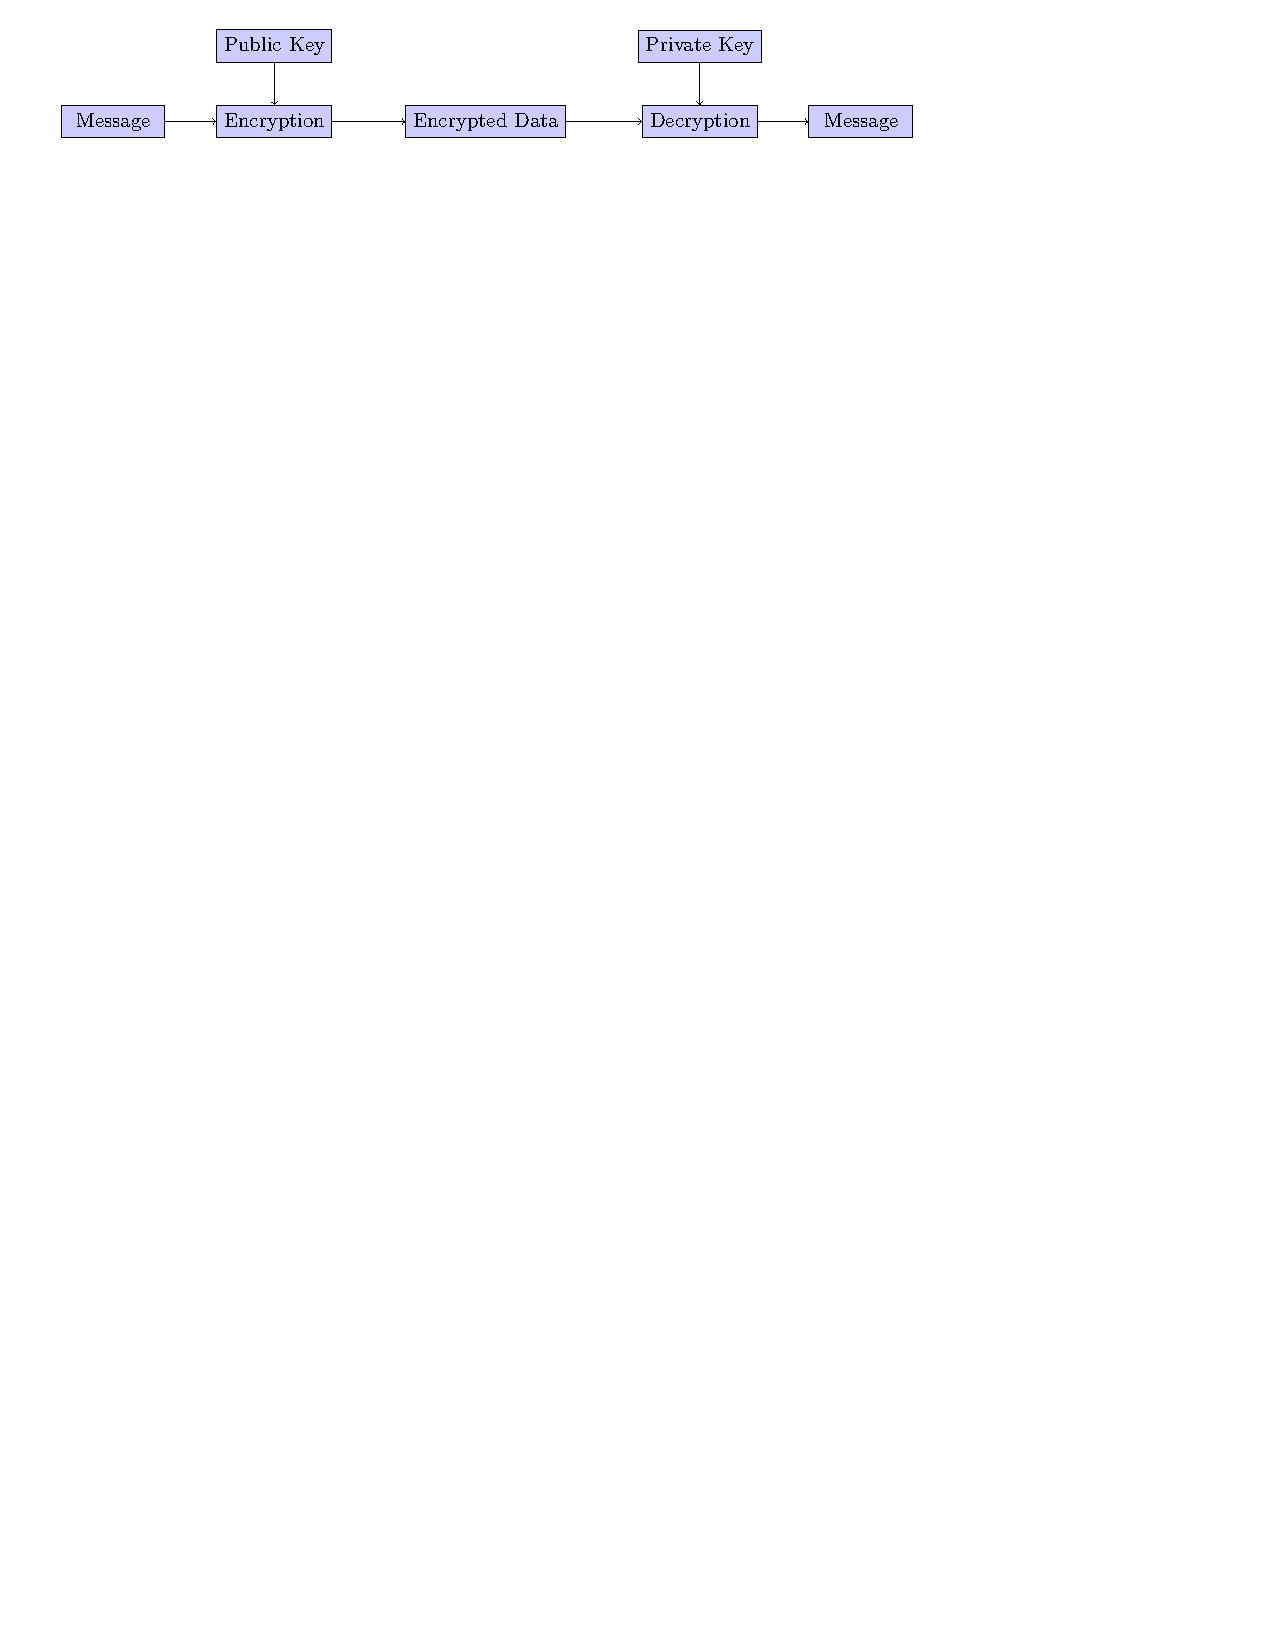
\includegraphics[trim=1cm 25.25cm 5cm 0cm]{figures/intro_asym_cipher.pdf}
\caption{Introduction of an asymmetric cipher operation}
\label{fig:asym}
%}
\end{figure}

Through the principle of private and public keys, asymmetric algorithms allow
privacy (like symmetric algorithm) but integrity of data too, because only this
one who creates the keys has the private key for decryption.

Three mains asymmetric cipher are used today:
\begin{itemize}
  \item RSA \cite{RFC3447} is currently the most widely used asymmetric
  cryptographic scheme, even though elliptic curves and discrete logarithms (see below) are gaining
  ground. The applications, which RSA is in practice the most used are:
  \begin{itemize}[noitemsep]
    \item Encryption of small pieces of data, especially for key transport
    \item Digital signatures (see section \ref{intro_sign})
  \end{itemize}
  
  \item Diffie-Hellman (DH) is a discrete logarithm (see section
  \ref{intro_secu}) which is most used in commercial cryptographic protocol like
  Secure Shell (SSH) \cite{RFC5647}, TLS \cite{RFC5246}, and Internet Protocol Security
  (IPSec) \cite{RFC3602}
  \item Elliptic Curve Diffie-Hellman (ECDH) is based on the conventional
  Diffie-Hellman explained above but using elliptic curves (see
  section \ref{intro_secu})
\end{itemize}

\section{Security of cryptographic algorithms}
\label{intro_secu}

All the keys use in cryptography have different sizes and different number of
parameters to generate the key.
These differences make the security level of each key algorithm.
The security level (in bits) of a key algorithm corresponds to the number of
operations needed ($2^{nbits}$) to break the security of it, meaning to find the
solution of the operation for the key calculation.

Table \ref{tab:intro_secu} shows the different security level of the main
cryptosystems existing in cryptography. We can see that an 80-bit symmetric key
provides roughly the same security as a 1024-bit RSA key.\newline

\begin{tabular}{|l|l|*{4}{r|}}
 \hline
 Algorithm Family	& Cryptosystems & \multicolumn{4}{|c|}{Security Level (bit)}\\
 					&				& 80 & 128 & 192 & 256 \\
 \hline
 Integer factorization & RSA & 1024	bits & 3072 bits & 7680 bits & 15360 bits \\
 Discrete logarithm & DH, DSA, Elgamal & 1024 bits & 3072 bits & 7680 bits &
 15360 bits \\
 Elliptic curves & ECDH, ECDSA & 160 bits & 256 bits & 384 bits & 512 bits \\
 \hline
 Symmetric-key & AES, 3DES & 80 bits & 128 bits & 192 bits & 256 bits \\
 \hline

\end{tabular}
\captionof{table}{Table of security level of each key algorithm}
\label{tab:intro_secu}


\subsection*{Symmetric key}

The security level of a symmetric key depends on the block cipher mode
operation chosen (see Section \ref{intro_sym_cipher}).

\subsection*{Integer factorization}

Integer factorization has the property to be based on large integers. This is
used for the RSA algorithm.
Compared to a symmetric algorithm, a RSA algorithm is several times slower. This
is because of the many computations involved in performing RSA.
A RSA is composed of a public exponent, a private exponent and a modulus.

\subsection*{Discrete logarithm}

Several algorithms are based on discrete logarithms problems in finite fields.
Diffie-Hellman and Digital Signature Algorithm (DSA) are examples of
discrete logarithms.

For the Diffie-Hellman a prime and a generator are needed to use this algorithm.
The length of the prime should be similar to the modulus of the RSA to provide
strong security. The generator should be a primitive element.
The prime and the generator represent the domain parameters of the
Diffie-Hellman algorithm.

For the Digital Signature Algorithm (DSA) a prime, a divisor and a generator are
needed to use this algorithm. Only the length of the prime and the divisor
provide different security level of the DSA algorithm. This is shown table
\ref{tab:intro_dsa_secu}.
The prime is represented by p and the divisor by q. The generator represents the
subgroups with q elements.
The prime, divisor and generator represent the domain parameters of the DSA
algorithm.\newline

\begin{center}
\begin{tabular}{|*{4}{c|}}

\hline
p		&	q	& Output (bits)	& Security levels \\
\hline
1024	&	160	& 160 			&	80 \\
2048	&	224	& 224 			&	112 \\
3072	&	256	& 160 			& 	128	\\
\hline

\end{tabular}
\captionof{table}{Table of security levels of DSA domain parameters}
\label{tab:intro_dsa_secu}

\end{center}

\subsection*{Elliptic Curves}

The Elliptic curves is the newest member of the three families of establishes
public-key algorithms. It provides the same level of security as Integer
factorizations or Discrete logarithms with shorter operands (see table
\ref{tab:intro_secu}). Elliptic curves are based on the generalized discrete
logarithm problem, that's why it can be used with Diffie-Hellman or DSA
protocol.

Elliptic curve Diffie-Hellman (ECDH) uses the same principle as standard
Diffie-Hellman, only the domain parameters change. For a ECDH algorithm an
elliptic curve should be used instead of the domain parameters. Several
elliptic curves are normalized \cite{RFC4492} and should be used in order to be
secure.

Elliptic curve Digital Signature Algorithm (ECDSA) uses the same principle as
standard DSA, only the domain parameters change. For a ECDSA algorithm an
elliptic curve should be used instead with a prime order. Table
\ref{tab:intro_ecdsa_secu} shows the security level of ECDSA.\newline

\begin{center}
\begin{tabular}{|*{3}{c|}}

\hline
q	& Output (bits)	& Security levels \\
\hline
192	& 192			&	96  \\
224	& 224 			&	112 \\
256	& 256 			& 	128	\\
384 & 384			&  	192 \\
512	& 512			&	256 \\
\hline

\end{tabular}
\captionof{table}{Table of security levels of ECDSA domain parameters}
\label{tab:intro_ecdsa_secu}

\end{center}

\newpage